\chapter{Implementation}

\paragraph{}
This section presents the work that has been done on the implementation.
We start by touching a few words on which variations have been used and what has been done before implementing our algorithm in parallel.
After that, we explicit each step of the parallel implementation, what has been implemented by hand and the parts that come from a library.
Finally, we present our experiments, the results and discuss them.

\section{Algorithm details}

\paragraph{Variations}
In our algorithm, we use spatially uniform sampling for the ease of implementation and robustness.
The kernel function is the bilateral function with the spatial parameter \(h_x = 40\) and the color intensity parameter \(h_z = 20\).
We use the re-normalised Laplacian \(\Lapl = \alpha (D-K)\)from \cite{milanfar_new_2016} to avoid expensive computation and use a simple definition.

\paragraph{Prototyping}
Initially, we implemented the algorithm proposed by \cite{glide_2014} in Python, using Numpy, in order to understand the mechanisms and issues of global filtering.
After that, we wrote our adapted algorithm in Python again, as a quick proof of concept.
Needless to say that this implementation is sequential and limited to small images that require only little computational resources.

\section{Parallel implementation}

\paragraph{}
To scale our algorithm to use usual camera pictures, but also much larger inputs, we implemented it in a parallel manner using the C language and the Portable, Extensible Toolkit for Scientific Computation (PETSc) \cite{petsc_web_page}.
This library is built upon MPI and contains distributed data structures and parallel scientific computation routines.
The most useful are the matrix and vector data structures and the parallel matrix-matrix and matrix-vector products.
Additionally, PETSc provides Krylov subspace methods and preconditioners for solving linear systems, also implemented in a scalable and parallel manner.
In a nutshell, PETSc provides an impressive parallel linear algebra toolkit, very useful to shorten the development time.
As we are basically using MPI, the main parallelism technique that we apply is SPMD.
It is possible to activate some SIMD parallelism with PETSc but we do not consider it in our case.
We want to point out to the reader that the distributed PETSc matrix data structure splits the data without overlap in a row-wise distribution manner.
In order to verify the correctness of our implementation, we used the Scalable Library for Eigenvalue Problem Computation (SLEPc) \cite{hernandez_slepc_2005}, which is based on PETSc and provides parallel eigenvalue problem solvers.
Furthermore, we need the library Elemental \cite{poulson_elemental_2013} in order to achieve dense matrix operations in PETSc.

We present how we included parallelism in our algorithm step-by-step, starting with reading the image and sampling.
Then follows the computation of the affinities of the sampled pixels.
And we finish with the computation of the smallest eigenvalues using the inverse subspace iteration.
The implementation associated to this project is open source and can be found on GitHub\footnote{\url{https://github.com/David-Wobrock/image-processing-graph-laplacian/}}.

\paragraph{Initialisation and sampling}
During the initialisation phase, the input image is read into memory sequentially by process 0.
Since we consider that the input image fits into memory, we broadcast the entire image from process 0 to all other processes.
Every process will hold the entire input image which will be useful since every process needs every pixel to compute the affinities.

The sampling step is also done by every process independently in a deterministic way.
All processes know the indices of the sampled pixels.
This is possible because we use spatially uniform sampling, which is deterministic, fast to compute and doesn't require communication.

\paragraph{Submatrices computations}
The computation of the affinity submatrices \(K_A\) and \(K_B\) is done locally by each process.
Indeed, each process computes the rows of the matrix that it will hold locally.
In other words, each process computes the affinities between a continuous subset of the sampled pixels and all pixels.
Since every process holds the complete image, no communication is needed.
The overhead is thus minimal and this part of the algorithm scales very well with respect to the number of processes.

Then, we compute the Laplacian submatrices \(\Lapl_A\) and \(\Lapl_B\).
The submatrix \(\Lapl_A\) requires to first compute the part \(D_A\) of the diagonal matrix \(D\) of normalisation coefficients.
Again, each process can locally sum each row of \(K_A + K_B\) because they have the same distribution layout, so no communication is needed.
However, to compute the normalisation factor \(\alpha\) in our Laplacian definition \(\alpha (D - K)\) with \(\alpha = \bar{d}^{-1}\) and \(\bar{d} = \sum^N_{i=1} \frac{d_i}{N}\), we need communication to find the average of the normalisation coefficients.
Nevertheless, the implied communication costs are not critical since we broadcast only one value for each process.

\paragraph{Inverse subspace iteration}
The algorithm to compute the smallest eigenvalues we use is the inverse subspace iteration inspired by \cite{el_khoury_acceleration_2014}.
With \(m\) the number of eigenvalues we will compute, \(p\) the sample size and \(m \le p\), we start the algorithm by selecting \(m\) random orthonormal independent vectors \(X_0\) of size \(p\).
We implemented a parallel Gram-Schmidt orthonormalising routine, based the classical sequential one.

The inverse iteration algorithm consists of outer and inner iterations, with \(k\) the index of the current outer iteration index.
The inner iteration consists of solving \(m\) linear systems, one for each vector of \(X_k\) that we approximate, such that \(\forall i \in [1, m]\) and \(X_k^{(i)}\) the \(i\)th vector of the subspace \(X_k\):
\[A X_{k+1}^{(i)} = X_k^{(i)}.\]
The outer iteration consists of repeating this process until convergence, meaning having a small enough residual norm.
We define the residual \(R_k\) of \(X_k\), at a certain iteration \(k\), as
\[R_k = A X_k - X_k X_k^T A X_k = (I - X_k X_k^T) A X_k.\]
A summary of the inverse subspace iteration algorithm:

\begin{algorithm}[H]
 \caption{Inverse subspace iteration}
 \begin{algorithmic}
  \REQUIRE \(A\) the matrix of size \(p \times p\), \(m\) the number of required eigenvalues, \(\varepsilon\) required precision of the subspace
  \ENSURE \(X_k\) the desired invariant subspace
  \STATE Initialise \(m\) random orthonormal vectors \(X_0\) of size \(p\)
  \STATE For k=0, 1, 2, \dots
  \WHILE{\(\|R_k\| > \varepsilon\)}
   \FOR{i=1 \TO m}
    \STATE Solve \(A X_{k+1}^{(i)} = X_k^{(i)}\)
   \ENDFOR
   \STATE Orthonormalise \(X_{k+1}\)
  \ENDWHILE
 \end{algorithmic}
\end{algorithm}

Solving the systems of linear equations is done using the Krylov type solvers and the preconditioners included in PETSc.
As a standard approach, we use the Restricted Additive Schwarz (RAS) method as preconditioning method, without overlap and 2 domains per process.
Each subdomain is solved using the GMRES method.

On each outer iteration, we must compute the residuals to see if we converged.
This is requires multiple matrix-matrix products and computing a norm, so communication cannot be avoided here.

\paragraph{Nystr\"om extension and output image}
As stated before, the Nystr\"om extension finds the leading eigenvectors, whereas we would need the trailing ones, as explains the articles \cite{belongie_spectral_2002}, \cite{fowlkes_spectral_2004} and \cite{glide_2014}.
So the algorithm will not compute the output image for now.

\section{Results}

\paragraph{Experimental setup}
The experiments to see how the algorithm scales are done on the test supercomputer of the Laboratoire Jacques-Louis Lions at Sorbonne Université.
This computer has 32 CPUs of 10 cores each and a total memory of 2 TB.
The setup of the experiments consists of running a specific test with different parameters, scaling the algorithm up to 250 processors.
The code is compiled on this computer using GCC 6.3.0 and the MPI implementation is Open MPI 1.8.3.
The versions of other libraries are PETSc 3.8.3, SLEPc 3.8.2 and Elemental 0.87.7.

\paragraph{}
We start by executing the algorithm without approximation.
This way, we will be able to see the results of the algorithm, even if the size of the input images will be limited.
After that, we study the approximation and computation of the smallest eigenvalues of the Laplacian.

\subsection{Entire matrix computations}

\paragraph{Results}
We start by showing the result of the computation using the full matrices.
We limited ourselves to grayscale images for the beginning and for computing the entire matrices, we can only process small images.
The image below is of size \(350 \times 350\), 122 500 pixels, so each matrix taking around 120 GB.

\begin{figure}[H]
  \centering
  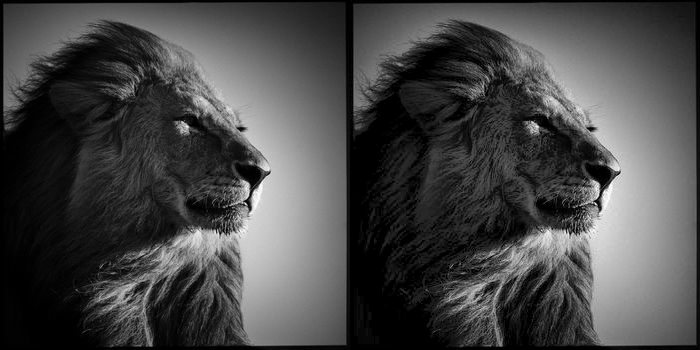
\includegraphics[width=0.95\textwidth]{img/lion.png}
  \caption{Left: input image. Right: sharpened image.}
\end{figure}

We observe more details on the lion's head and the mane on the left-hand side appears brighter.
However, the already detailed parts are not over-sharpened.
The sharpening is done by defining the output image as \(z = (I - f(\Lapl))y\) with, in this case, \(f(\Lapl) = -3\Lapl\).
We fall back on the adaptive sharpening operator defined in \cite{siam_slides_2016} as \((I + \beta \Lapl)\) with \(\beta > 0\).

\paragraph{Performances and discussions}
We run the algorithm 5 times for each number of processors, on the image shown above, from 8 to 128 processors for each power of 2.
First, the total runtime for each number of processors:
\begin{figure}[H]
  \centering
  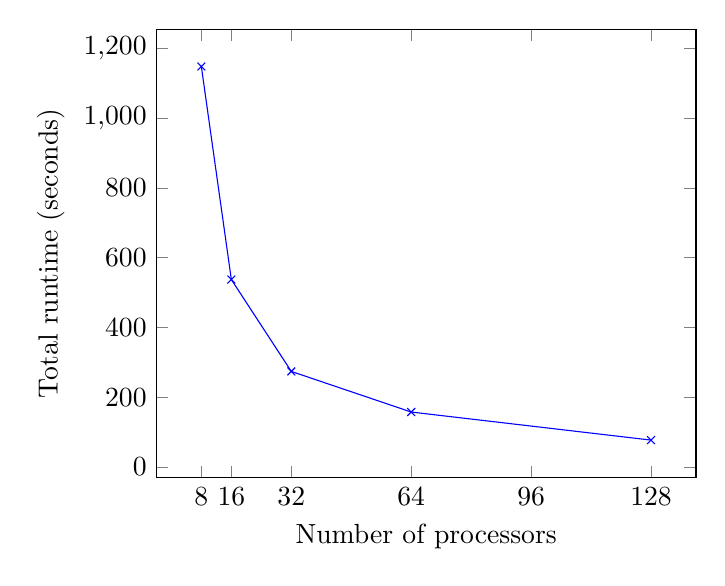
\begin{tikzpicture}
   \begin{axis}[
    xlabel=Number of processors,
    xtick={8, 16, 32, 64, 96, 128, 150},
    ylabel=Total runtime (seconds)]
     \addplot[color=blue, mark=x] coordinates {
      (8, 1148.389)
      (16, 537.521)
      (32, 274.0227)
      (64, 157.5765)
      (128, 77.0977)
     };
   \end{axis}
  \end{tikzpicture}
  \caption{Total runtime of the algorithm with entire matrix computation.}
\end{figure}

We observe that the runtime decreases significantly with respect to the number of processors.
We can also see that, by doubling the number of processors, we nearly accelerate the runtime by a factor 2.
It is one of the best result we could expect since we achieved strong scalability for the entire matrix computation case.
However, some overhead will always be present and the matrix-vector operations necessarily require communication, limiting scalability.
To observe if some parts scale better than others, we compare the proportion of each part:
\begin{figure}[H]
  \centering
  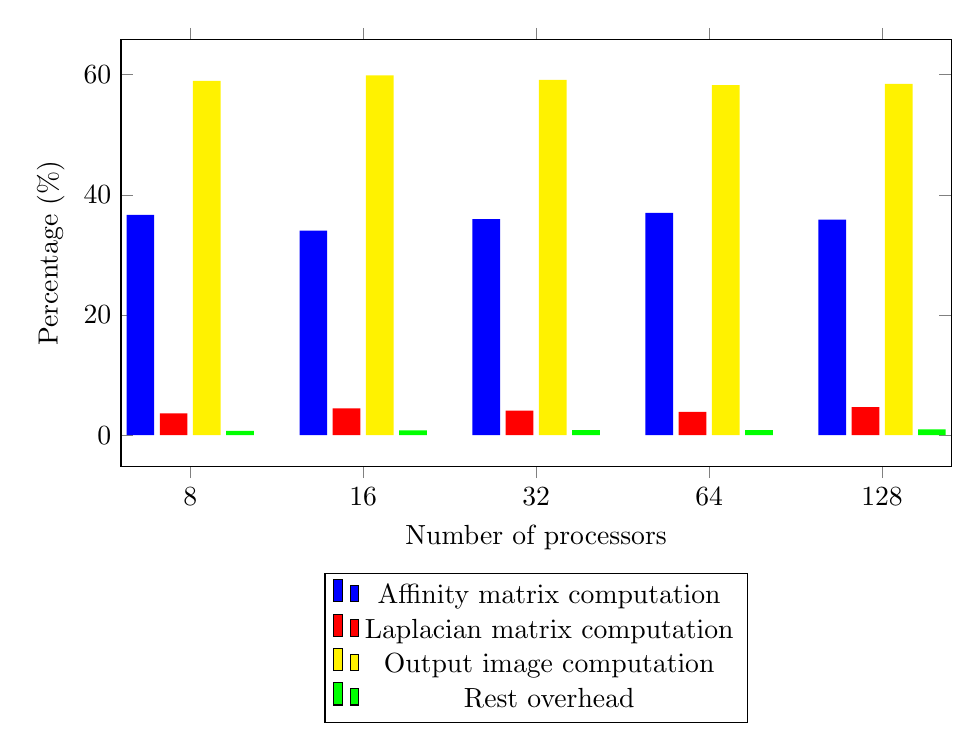
\begin{tikzpicture}
   \begin{axis}[
    ybar,
    height=7cm,
    width=\textwidth,
    xlabel=Number of processors,
    xtick={0, 1, 2, 3, 4},
    xticklabels={8, 16, 32, 64, 128},
    legend style={
     at={(0.5, -0.25)},
     anchor=north
    },
    ylabel={Percentage (\%)}]
    \addplot[draw=none, fill=blue] coordinates {
     (0, 36.67)
     (1, 34.04)
     (2, 35.96)
     (3, 37)
     (4, 35.88)};
    \addplot[draw=none, fill=red] coordinates {
     (0, 3.62)
     (1, 4.48)
     (2, 4.07)
     (3, 3.88)
     (4, 4.67)};
    \addplot[draw=none, fill=yellow] coordinates {
     (0, 58.99)
     (1, 59.9)
     (2, 59.15)
     (3, 58.26)
     (4, 58.48)};
    \addplot[draw=none, fill=green] coordinates {
     (0, 0.72)
     (1, 0.78)
     (2, 0.82)
     (3, 0.86)
     (4, 0.96)};
    \legend{Affinity matrix computation,
     Laplacian matrix computation,
     Output image computation,
     Rest overhead}
   \end{axis}
  \end{tikzpicture}
  \caption{Proportion of each step in the total execution of the algorithm with entire matrix computation.}
\end{figure}

We see that the proportion of each part remains the same, meaning that the three main parts, in this interval of number of processors, scale equivalently.
When allocating an excessive amount of processors to this task, it may be that we observe an increase of the runtime because we spend time communicating.

\subsection{Approximation computations}

\paragraph{Eigenvalues}
We remind that the end of the algorithm, using matrix approximations to compute the filtered image, is not implemented.
Nonetheless, we will present interesting results about the computation of the eigenvalues of the graph Laplacian operator.

\paragraph{Performances}
TODO

\paragraph{SLEPc comparison}
TODO
